%!TEX program = xelatex
\documentclass[9pt, compress]{beamer}
\usetheme[titleprogressbar]{m}

\usepackage{array}
\usepackage{tabu}
\usepackage{longtable} %tabu needs this to be loaded.
\usepackage{lipsum}
\usepackage{multicol}
\usepackage{rotating}

\usepackage{color}
\usepackage{xcolor}
\usepackage{listings}
\usepackage{sectsty}
\usepackage{caption}


\DeclareCaptionFont{white}{\color{white}}
\DeclareCaptionFormat{listing}{\colorbox{gray}{\parbox{\dimexpr\textwidth-1.72\fboxsep\relax}{#1#2#3}}}
\captionsetup[lstlisting]{format=listing,labelfont=white,textfont=white,margin=0pt}
\lstset{language=C,
	basicstyle=\footnotesize,
	keepspaces=true,
	tabsize=4,               
	frame=single,                           % Single frame around code
	rulecolor=\color{black},
	captionpos=b,
	showstringspaces=false,	
	abovecaptionskip=-0.9pt,
	xleftmargin=3.4pt,
	xrightmargin=2.6pt,
	breaklines=true,
	postbreak=\raisebox{0ex}[0ex][0ex]{\ensuremath{\color{black}\hookrightarrow\space}},
	xleftmargin=3.2pt,
	escapechar=\&,
	literate={а}{{\selectfont\char224}}1
	{~}{{\textasciitilde}}1
	{б}{{\selectfont\char225}}1
	{в}{{\selectfont\char226}}1
	{г}{{\selectfont\char227}}1
	{д}{{\selectfont\char228}}1
	{е}{{\selectfont\char229}}1
	{ё}{{\"e}}1
	{ж}{{\selectfont\char230}}1
	{з}{{\selectfont\char231}}1
	{и}{{\selectfont\char232}}1
	{й}{{\selectfont\char233}}1
	{к}{{\selectfont\char234}}1
	{л}{{\selectfont\char235}}1
	{м}{{\selectfont\char236}}1
	{н}{{\selectfont\char237}}1
	{о}{{\selectfont\char238}}1
	{п}{{\selectfont\char239}}1
	{р}{{\selectfont\char240}}1
	{с}{{\selectfont\char241}}1
	{т}{{\selectfont\char242}}1
	{у}{{\selectfont\char243}}1
	{ф}{{\selectfont\char244}}1
	{х}{{\selectfont\char245}}1
	{ц}{{\selectfont\char246}}1
	{ч}{{\selectfont\char247}}1
	{ш}{{\selectfont\char248}}1
	{щ}{{\selectfont\char249}}1
	{ъ}{{\selectfont\char250}}1
	{ы}{{\selectfont\char251}}1
	{ь}{{\selectfont\char252}}1
	{э}{{\selectfont\char253}}1
	{ю}{{\selectfont\char254}}1
	{я}{{\selectfont\char255}}1
	{А}{{\selectfont\char192}}1
	{Б}{{\selectfont\char193}}1
	{В}{{\selectfont\char194}}1
	{Г}{{\selectfont\char195}}1
	{Д}{{\selectfont\char196}}1
	{Е}{{\selectfont\char197}}1
	{Ё}{{\"E}}1
	{Ж}{{\selectfont\char198}}1
	{З}{{\selectfont\char199}}1
	{И}{{\selectfont\char200}}1
	{Й}{{\selectfont\char201}}1
	{К}{{\selectfont\char202}}1
	{Л}{{\selectfont\char203}}1
	{М}{{\selectfont\char204}}1
	{Н}{{\selectfont\char205}}1
	{О}{{\selectfont\char206}}1
	{П}{{\selectfont\char207}}1
	{Р}{{\selectfont\char208}}1
	{С}{{\selectfont\char209}}1
	{Т}{{\selectfont\char210}}1
	{У}{{\selectfont\char211}}1
	{Ф}{{\selectfont\char212}}1
	{Х}{{\selectfont\char213}}1
	{Ц}{{\selectfont\char214}}1
	{Ч}{{\selectfont\char215}}1
	{Ш}{{\selectfont\char216}}1
	{Щ}{{\selectfont\char217}}1
	{Ъ}{{\selectfont\char218}}1
	{Ы}{{\selectfont\char219}}1
	{Ь}{{\selectfont\char220}}1
	{Э}{{\selectfont\char221}}1
	{Ю}{{\selectfont\char222}}1
	{Я}{{\selectfont\char223}}1,
	extendedchars=true
}
\usepackage{textpos}
\newcommand<>{\fullsizegraphic}[1]{
  \begin{textblock*}{0cm}(-0.9cm,-3.78cm)
  \includegraphics[width=\paperwidth]{#1}
  \end{textblock*}
}

%галочка
\usepackage{amssymb}% http://ctan.org/pkg/amssymb
\usepackage{pifont}% http://ctan.org/pkg/pifont
\newcommand{\cmark}{\ding{52}}%
\newcommand{\xmark}{\ding{56}}

\usepackage{booktabs}  
\usepackage[scale=2]{ccicons}
\usepackage{minted}
\usepgfplotslibrary{dateplot}
\usemintedstyle{trac}
\author{Студент: \textbf{Д.В. Круминьш}\\ 
	Группа: \textbf{13541/3}\\ \\
	Преподаватель: \textbf{И.А. Малышев} } 
\title{Отчет о лабораторной работе №4}
\subtitle{Курс: \textbf{Администрирование компьютерных сетей}\\
Тема: \textbf{Устранение уязвимостей}}
%\logo{123}
\institute{Санкт-Петербургский политехнический университет Петра Великого}
\date{ }
%\subject{}
%\setbeamercovered{transparent}
%\setbeamertemplate{navigation symbols}{}
\begin{document}
	\maketitle
%	\begin{frame}
%		\frametitle{Оглавление}
%		\tableofcontents{}
	%\end{frame}
\begin{frame}
\frametitle{Цели работы}
\begin{enumerate}
\item Устранение найденных уязвимостей хостов в сети.
\end{enumerate}
\end{frame}


\begin{frame}
\frametitle{Схема компьютерной сети}
\begin{center}  
	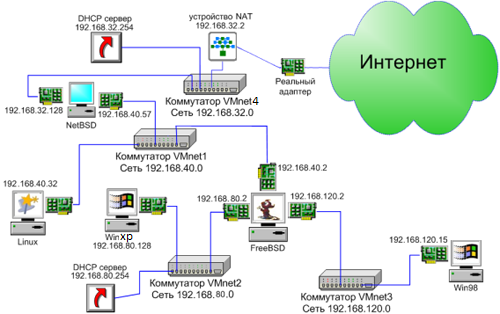
\includegraphics[width=\textwidth]{img/KKS_full}
\end{center}
\end{frame}

\begin{frame}
\frametitle{Найденные уязвимости}
Ранее были выявлены следующие уязвимости:
\begin{itemize}
\item Windows XP (192.168.80.128)
\begin{itemize}
\item сервисом NTP открыт порт 123 по UDP;
\item сервисом RPC Windows открыт порт 135 по TCP;
\item сервисом NBNS открыт порт 137 по UDP;
\item сервисом NetBIOS открыт порт 139 по TCP.
\end{itemize}
\item Windows 98 (192.168.120.15)
\begin{itemize}
\item сервисом NetBIOS-SSN открыт порт 137 по UDP;
\item сервисом NetBIOS открыт порт 139 по TCP.
\end{itemize}
\end{itemize}
\end{frame}


\begin{frame}
\frametitle{Способы устранения уязвимостей}
Устранить данные уязвимости можно следующими способами:
\begin{enumerate}
\item установка патчей безопасности;
\item редактирование реестра и системных настроек;
\item настройка межсетевого экрана.
\end{enumerate}
В данном случае будет настроен межсетевой экран, который будет настроен на хосте с FreeBSD.
\end{frame}


\begin{frame}[fragile]
\frametitle{Устранение уязвимостей}
Внесем следующие настройки в файл \textbf{/etc/rc.conf}:
\begin{lstlisting}[language={}]
firewall_enable="YES"
firewall_type="/usr/fw_rules/ruleFile"
\end{lstlisting}
Первой строчкой включается межсетевой экран, а второй файл с фильтрами.
\end{frame}


\begin{frame}[fragile]
\frametitle{Устранение уязвимостей}
В созданный файл \textbf{/usr/fw\_rules/ruleFile} внесем следующие строчки:
\begin{lstlisting}[language={}]
# Windows XP
add deny udp from any to 192.168.80.128 123
add deny tcp from any to 192.168.80.128 135
add deny udp from any to 192.168.80.128 137
add deny tcp from any to 192.168.80.128 139

# Windows 98
add deny udp from any to 192.168.120.15 137
add deny tcp from any to 192.168.120.15 139

# Allow all other packets
add allow in
add allow out
\end{lstlisting}
Данными правилами были заблокированы пакеты, которые могут использовать уязвимости.

После этого необходимо перезагрузить систему.
\end{frame}


\begin{frame}[fragile]
\frametitle{Проверка}
В качестве проверки можно использовать утилиту \textbf{telnet}. Например, проверим доступность порта 139 до включения экрана:
\begin{center}  
	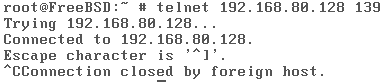
\includegraphics[width=.6\textwidth]{img/1}
\end{center}
После включения экрана:
\begin{center}  
	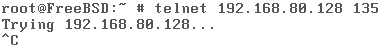
\includegraphics[width=.6\textwidth]{img/2}
\end{center}
Как и ожидалось, установить соединение с выбранным портом не удалось.
\end{frame}

\begin{frame}[fragile]
\frametitle{Вывод}
В данной работе были рассмотрены возможности по устранению уязвимостей ОС.

Наилучшим решением будет являться установка последних патчей безопасности, но это не всегда возможно. 

Более оперативным и гибким решением является настройка межсетевого экрана, что и было сделано в данной работе.
\end{frame}	
	

	
\end{document}
